The Standard Model in particle physics encompasses all of the
Elementary particles and their interactions. It is a gauge theory spontaneously broken by the Higgs mechanism with the gauge group $ SU(3)_C \otimes SU(2)_L \otimes U(1)_Y $.\\
From a theoretical point of view, the Standard Model is a quantum field theory based on local gauge invariance and consists of two rough parts. The electroweak sector $ SU(2)_L \otimes U(1)_Y $ is called GWS (Glashow-Weinberg-Salam) theory and describes the gauge bosons $ W^{\pm}, Z^0, \gamma $, the Higgs sector and its interaction with the leptons and quarks. In contrast to the other gauge bosons, the exchange particles of the weak interaction carry mass, which also affects the properties of the interactions. The colour-charged sector $ SU(3)_C $, the chromo dynamics, deals with quarks and contains the eight massless, electrically neutral gluons as gauge bosons. The gauge groups $SU(3)_C$ and $SU(2)_L$ are 
non-abel gauge theories, more precisely Yang Mills theories.
The massive particles, fermions, will be divided into two groups, leptons and quarks. Each group is arranged in 3 generations. Within the leptons there are three electrically neutral neutrinos. The mass of the particles increases from generation to generation. Neutrinos only interact weakly, whereas the charged leptons interact both weakly and electromagnetically. Quarks are characterised by the fact that they can also interact strongly \cite{edelhaeuser2016tutorium}. 

\section{Quantum chromo dynamics}

Overall, there are four types of interactions.\\


\begin{tabular}{|c|c|c|c|c|}
\hline 
Interaction & Energy scale & Range [m] & Mediators \\ 
\hline 
Strong & $ \sim 1 $  & $10^{-15} $ & $g$ \\ 
\hline 
Electromagnetic & $ \sim 10^{-2} $ & $\infty$ & $\gamma $ \\ 
\hline  
Weak & $ \sim 10^{-6} $ & $10^{-18}$ & $W^{\pm}, Z$ \\ 
\hline
Gravity & $ \sim 10^{-38} $ & $\infty$ & maybe graviton \\ 
\hline 
\end{tabular}  
\\
\\
\\
Nucleons are made up of quark and gluons called partons.
Whereby, the gluons are the exchange bosons for this short ranged interaction.
\begin{figure}[h!]
\centering
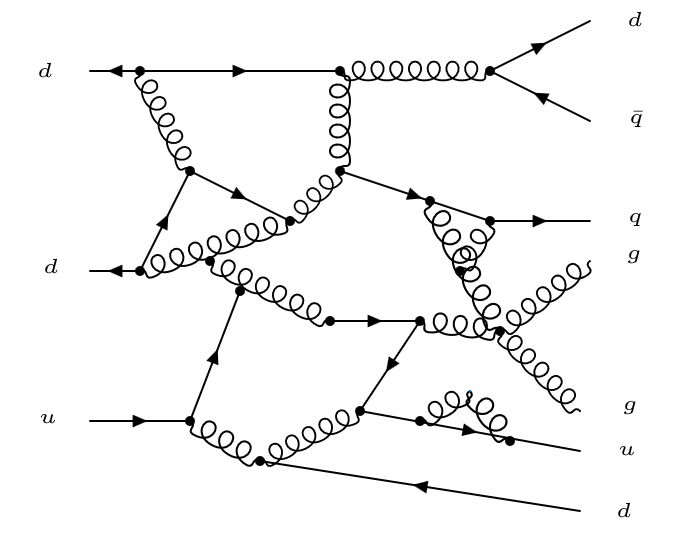
\includegraphics[scale=0.8]{images/Intro/Neutron.png}
\caption{A schematic picture of neutron structure. at the left side of the resolution is too low to see. The 3 quarks picture allows us to interpretate the quantum numbers of the neutron in the valence band.
In high-resolution picture for a large $ Q^2 $ can be obtained a gluon sea and a lot of quarks pairs\cite{Cunha13}. The quantum number of a neutron is for each energy scale the same}.
\end{figure}
To explain the short range of the strong interaction Yukawa (1934) postulated mesons as a mediator for the nuclear force by the exchange of this massive field quanta. Three years later a candidate ($ \pi $ meson) was found in cosmic rays. Later on it was shown massive field quanta break the gauge symmetry so that the mediator must be massless. If it is based on the SU(3) gauge symmetry of the QCD massless Lagrangian how can the strong sector be short range? Another question came from a series of experiments at SLAC. Through high-energy electron-proton scattering there was a search for evidence of the existence of quarks and their behaviour like free particles despite the energetically bound inner proton. The solution to these question was explained by Gross, Politzer and Wilczek through asymptotic freedom. 
This effect can be proved by the running coupling and anti screening in QCD.
For the calculation of the propagator loop correction in QCD both quark loops (negative contribution $ \rightarrow $ screening) and gluon loops (positive contribution $ \rightarrow $ anti screening) have to be taken into account. 
\begin{figure}[h!]
\centering
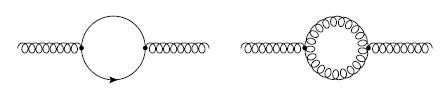
\includegraphics[scale=0.7]{images/Intro/quarkGluonPop.png}
\caption{Running coupling compared for QED, with a positive and QCD with a negative beta function. The quark loop vacuum polarization diagram gives a negative contribution
to $\beta_0 \sim n_f$ and the gluon loop gives a positive contribution to $\beta_0 \sim N_c$. The second contribution is bigger than the first, so that $ \beta_0 > 0 $ in QCD. The beta function in QED is negative since the second contribution does not exist $ N_C=0 $.}
\end{figure}

The one loop running coupling in QCD is:
\begin{equation}
\begin{split}
\alpha_s(Q^2)= \frac{\alpha_s(\mu^2)}{1+\beta_0 \alpha_s(\mu^2) ln(\frac{Q^2}{\mu^2})}
\end{split}
\end{equation}
\\
\\
\pagebreak

Where $ \beta_0 = \dfrac{11N_c -2n_f}{12\pi} $, $ n_f $ the number of quarks comes from the first diagram and causes screening.  $ N_c $ the number of colours is due to anti screening. Obviously, with $ n_f = 6 $ and $ N_c = 3 $ in standard model we will get $ \beta_0 >0 $. The Beta function is defined as:
\begin{equation}
\begin{split}
\beta(\alpha)=-(\beta_0 \alpha^2 + \beta_1 \alpha^3+\beta_2\alpha^4+....)=\frac{d\:\alpha(Q^2)}{d \:ln(Q^2)}
\end{split}
\end{equation}

e.g. the first term of beta-function is negative in contrast to QED with $ \beta_0=- \dfrac{\pi}{3} \rightarrow -(\beta_0 \alpha^2) >0 $. The coupling constant in QCD will be increased
with reduction of $ Q^2 $ (increasing distance), in QED vice versa.
\begin{figure}[h!]
\centering
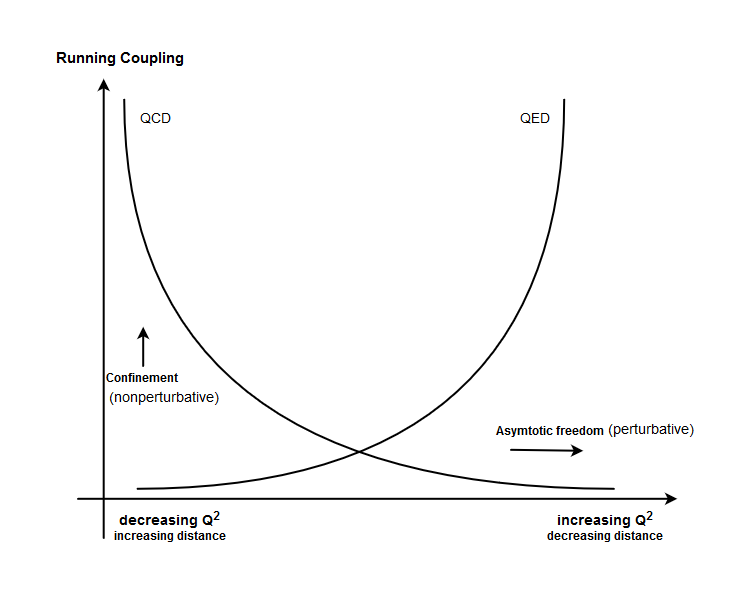
\includegraphics[scale=0.7]{images/Intro/QCDRunningCoupling.png}
\end{figure}



Asymptotic freedom allows us to use perturbation theory. Actually there is need of two more things to make the connection between theory and experiment: either infrared safety or factorisation. That is clarified in the next chapter\ref{Hard scattering}.
Quarks have not yet been observed as free particles. With increasing separation it will be easier to produce a quark-antiquark pair than to isolate a quark because the coupling between them is too strong. This mechanism is called confinement. Confinement as a non-perturbative theory has been confirmed in Lattice QCD, but not yet mathematically.
Quarks prefer to bind into hadrons which can be classified into baryons with three quarks state and mesons with a quark-antiquark state.
The wave function of fermions must be antisymmetric according to the Pauli exclusion principle under exchange of two quarks. Interestingly, there are resonance states with spin $ \frac{3}{2} $ like $ {\Delta}^{++} $.
The spins of the three up quarks are parallel to each other, have the same flavour and orbital angular momentum L=0. This means that an exchange of flavour, spin and space (orbital angular momentum) does not lead to any change. This problem was explained with the additional degree of freedom, the so-called color charge. This additional factor $N_C$ could be determined experimentally in the electron-positron annihilation into hadrons schematically in figure \ref{ratio}. 

\begin{figure}[h!]
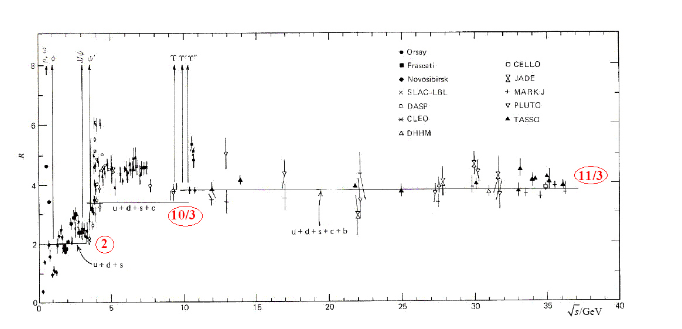
\includegraphics[width=1.1\textwidth, left]{images/Intro/Ratio.png}
\caption{Key measurement at lepton collider, $R = \frac{\sigma(e^+e^- \rightarrow Hadrons)}{\sigma(e^+e^- \rightarrow \mu^+ \mu^-)} =N_C \sum_q e^2_q$, evidence for $N_C=3$ colours of quarks. Without this factor the ration is for $ u, d, s $, $ u, d, s, c $ and $ u, d, s, c, b $ Respectively $ \frac{2}{3}, \frac{10}{9}, \frac{11}{10} $ The experiment showed a third of the expected results \cite{Eva}.}
\label{ratio}
\end{figure}


Each quark comes in one of three colours red, green or blue and also anti-colour $ \bar{r}, \bar{b}, \bar{g} $  for anti-quarks. The hadrons are colour singlets with regard to the hypothesis and so are invariant under rotations in colour space. The colour hypothesis describes the existence of mesons with $ q \bar{q} $ and baryons with $ qqq $. \\
The total wave function for each particle can be expressed:

\begin{equation}
\begin{split}
\Psi_{3q} &= \psi_{space} \times \chi_{spin} \times \theta_{colour} \times \phi_{flavour} \\
&\:\:\:\:\:\:\:O(3) \:\:\:\:\: SU(2)\:\:\:\: SU(3)\:\:\:\:\: SU(6)\\
\end{split}
\end{equation}
All possible colour states are described with Young Tableaux \cite{Greiner1989}. The group theory methods are used to decompose products of irreducible representations into sums for instance the Young Tableaux technique.
\begin{figure}[h!]
\centering
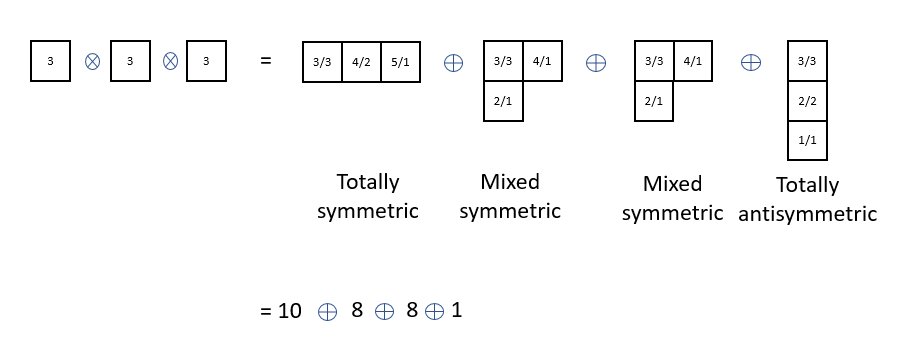
\includegraphics[scale=0.7]{images/Intro/Young.png}
\end{figure}

The same procedure for SU(2) and SU(6) for spins and flavours of the three quarks turns out:

\begin{equation}
\begin{split}
2\: \otimes\:2 \:\otimes\:2 &= 4 \:\:\:\oplus\: 2\:\:\:\oplus\:2\:\:\:\oplus\:0\\
6\: \otimes\:6 \:\otimes\:6&= 56 \:\oplus\: 70\:\oplus\:70\:\oplus\:20
\end{split}
\end{equation}


\pagebreak
\section{QCD Lagrangian}
\label{QCD Lagrangian}

QCD like QED and the weak interaction theory is described by representations of a symmetry group. From the condition that the Lagrangian must be invariant under arbitrary global and local symmetry transformations (Noether’s theorem) follows the interaction terms.
The Lagrangian of QCD is invariant under $ U(1) \times SU(3) $ global transformation. The three Pauli matrices from $ SU(2) $ can be replaced by the eight Gell-Mann $ \lambda^a $ with the following Lie algebra: 
\begin{equation}
\begin{split}
&T^a = \frac{1}{2} \lambda^a\\
&[T^a, T^b]= if^{abc} T^c \:\:\:\:\:\:\:\:\:\:\:\:\:\:\text{fundamental representation}\\
&({T^a}_{adj})_bc = -if^{abc} \:\:\:\:\:\:\:\:\:\:\:\:\text{adjoint representation}
\end{split}
\end{equation}
To quantize QCD theory, the Faddeev-Popov method \cite{Faddeev:1967fc} is usually used in the path integral to fix a gauge and define a gluon propagator. The Lagrangian is given:

\begin{equation}
\begin{split}
& \mathscr{L} = \sum_f \bar{\psi}_{if} (i\gamma^{\mu} {\partial}_{\mu}-m_f){\psi}^{jf}-\frac{1}{4}{F_a}^{\mu \nu}{F^a}_{\mu \nu}-\frac{1}{2\xi}(\partial^{\mu} {A^a}_{\mu})(\partial^{\nu} {A^a}_{\nu})+(\partial^{\mu} {\chi^a}^*)(\partial_{\mu} {\chi^a})\\
&{\color[RGB]{255,0,0} -g_s \bar{\psi}_{i} {T^a}_{ij}{\psi}_{j} \gamma^{\mu} {A^a}_{\mu}-\frac{g_s}{2} f^{abc}(\partial_{\mu} {A^a}_{\nu}-\partial_{\nu} {A^a}_{\mu}){A_b}^{\mu}{A_c}^{\nu})-\frac{{g_s}^2}{4} f^{abc} ({A_b}^{\mu}{A_c}^{\nu})f^{ade} ({A^d}_{\mu} {A^e}_{\nu})}\\
\\
&{\color[RGB]{255,0,0} -g_s f^{abc} (\partial^{\mu} {\chi^a}^{*}){\chi^b}{A^c}_{\mu}}\\
\end{split}
\end{equation}

The red marked part gives the Langrangian of free particles and the black part takes care of the interactions. ${F^a}_{\mu \nu}$ is field strength tensor for spin-1 gluon field $ {A^a}_{\mu} $ corresponded to a non-Abelian gauge theory with the structure constants $ f^{abc} $.

\begin{equation}
\begin{split}
{F^a}_{\mu \nu}= \partial_\mu {A^a}_{\nu}-\partial_\nu {A^a}_{\mu}-g_s f_{abc} {A^b}_{\mu} {A^c}_{\nu}
\end{split}
\end{equation}
The third term distinguishes QCD from QED, giving rise to triplet and quartic gluon self-interaction.
Here $i$, $j$ are color indices in the fundamental representation, $a, b , c$ run over 8 colour degrees of freedom of the gluon fields in the adjoint representation of SU(3). $f$ labels the six flavours of the quarks. $ g_s $ describes the strong coupling constant. Due to gauge fixing the Langrangian in the non-Abelian case requires the introduction of additional fields. These anti commuting complex scalar fields $ {\chi^a} $ are called Faddeev Popov ghosts \cite{Schwartz:2013pla, peskin2018introduction}. Feynman rules follows the Lagrangian. A list of the respective Feynman rules regarding the terms can be found in\ref{Math}  which will be used for the aims of this work later.

%
%\pagebreak
%It can be shown that the above Lagrangian is invariant under the following $ SU(3) $ gauge transformations:
%\begin{equation}
%\begin{split}
%&{\psi}^{\prime}(x) \rightarrow exp(i \:\eta_a(x) \:T^a) \:\psi(x)\\
%&{D}^{\prime} \rightarrow \partial_\mu+ig_sT_a\: {{A}^{\prime}}^a_{\mu } \\
%&{{A}^{\prime}}^a_{\mu }\rightarrow  {A^a}_{\mu}- \frac{1}{g_s}\partial_\mu \eta^a(x)+ f^{abc} \eta_{b}(x) {A_c}_{\nu}(x)
%\end{split}
%\end{equation}

\label{Feynman}

\pagebreak

\section{Colour factor calculation}
\label{col}
In this section the calculation of the Casimir operators of the respective diagrams is motivated, which occur later with the evaluation of the matrix elements. The generalization of the Pauli matrices are the so-called Gell-Mann matrices $\lambda ^a$ which is given by \cite{Schwartz:2013pla, Platzer:2018pmd}
\begin{equation}
\begin{split}
T^a = \vartheta^a \equiv \frac{\lambda ^2}{2}
\end{split}
\end{equation}

\begin{equation}
\begin{split}
\lambda ^1 =\begin{pmatrix} 0& 1 &\\ 1& 0 &\\ & & 0 \end{pmatrix},\:\:\: \lambda ^2 =\begin{pmatrix} 0& -i &\\ i& 0 &\\ & & 0 \end{pmatrix}, 
\:\:\: \lambda ^3 =\begin{pmatrix} 1&  &\\ & -1 &\\ & & 0 \end{pmatrix}, \:\:\: \lambda ^4 =\begin{pmatrix} &  &1\\ & 0&\\1 & &  \end{pmatrix}\\\
\lambda ^5 =\begin{pmatrix} &  &-i\\ & 0 &\\ i& &  \end{pmatrix},\:\:\: \lambda ^6 =\begin{pmatrix} 0&  &\\ & 0 &1\\ & 1& 0 \end{pmatrix}, 
\:\:\: \lambda ^7 =\begin{pmatrix} 0&  &\\ & 0 &-i\\ & i& 0 \end{pmatrix}, \:\:\: \lambda ^8 =\frac{1}{\sqrt3}\begin{pmatrix} 1&  &\\ & 1&\\ & &-2  \end{pmatrix}
\end{split}
\end{equation}
$ {\lambda}^3 $ and $  {\lambda}^8 $ are diagonal. These generators satisfy schematically:\\ 
\begin{itemize}
\item in the fundamental representation
\begin{figure}[h!]
\centering
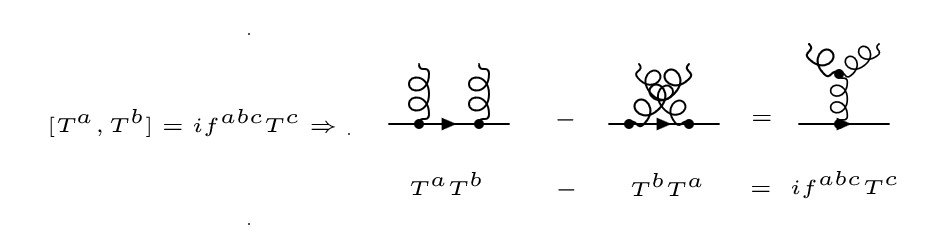
\includegraphics[scale=0.6]{images/Intro/Casimir.png}
\end{figure}
\item in the adjoint representation\\
\begin{figure}[h!]
\centering
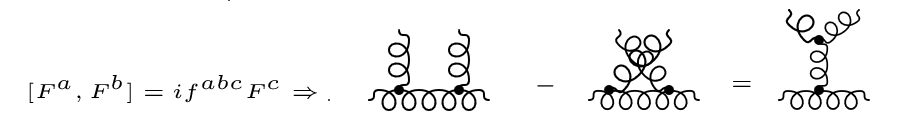
\includegraphics[scale=0.6]{images/Intro/CasimirAdj.png}
\end{figure}
\end{itemize}
\pagebreak
The most common convention for the normalization of the generators in physics is:
\begin{equation}
\displaystyle\sum\limits_{c,d} f^{acd} f^{bcd} = N \delta^{ab}
\end{equation}
One of the most important equations for the colour factor calculation is the Jaccobi-Identity:
\begin{equation}
\begin{split}\:
[T^a, [T^b , T^c]]+[T^c, [T^a , T^b]]+[T^b, [T^c , T^a]]=0
\end{split}
\end{equation}
In terms of the structure constant:
\begin{equation}
\begin{split}\:
f^{axd} f^{bcx} +  f^{cxd} f^{abx} +f^{bxd} f^{cax} =0
\end{split}
\end{equation}

\begin{equation}
f^{abc} = -2i\: tr(T^a[T^b, T^c])
\end{equation}
Which generalises to:
\begin{equation}
f^{abc}f^{xcd} = 4i\: tr(T^a[T^b, [T^c, T^d]])
\end{equation}

With these relations all Casimir operators can be calculated:\\
\begin{itemize}
\item Fundamental representation Casimir operator\\
\begin{figure}[h!]
\centering
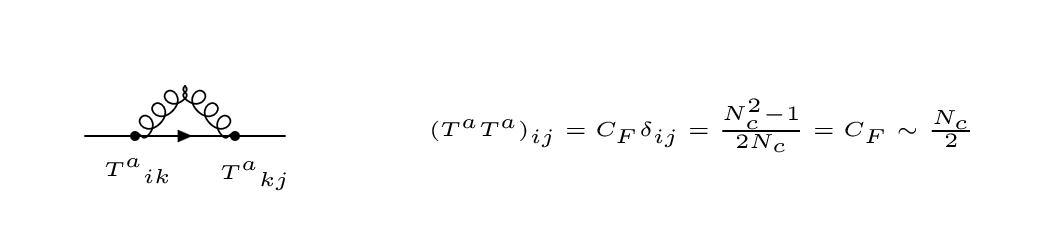
\includegraphics[scale=0.6]{images/Intro/Casimir1.png}
\end{figure}
\item Adjoint representation Casimir operator\\
\begin{figure}[h!]
\centering
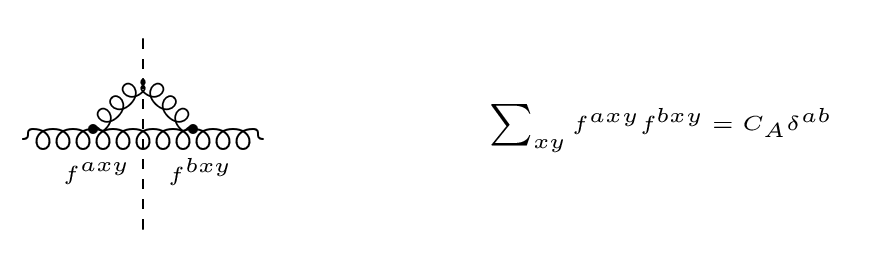
\includegraphics[scale=0.6]{images/Intro/Casimir2.png}
\end{figure}
\pagebreak
\\

Which means the charge of the gluon is twice that of the quark because:
\begin{equation}
 C_A = N_c =2C_F \sim 2(\frac{N_C}{2}) 
\end{equation}
\item Trace identities:\\
\begin{figure}[h!]
\centering
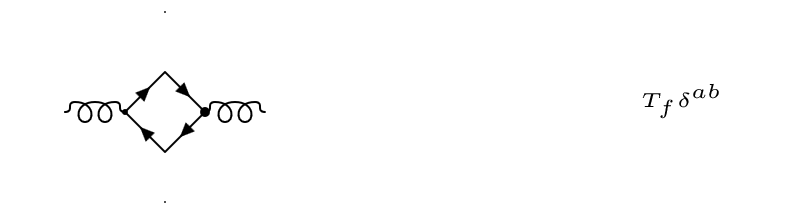
\includegraphics[scale=0.6]{images/Intro/Casimir3.png}
\end{figure}
\begin{figure}[h!]
\centering
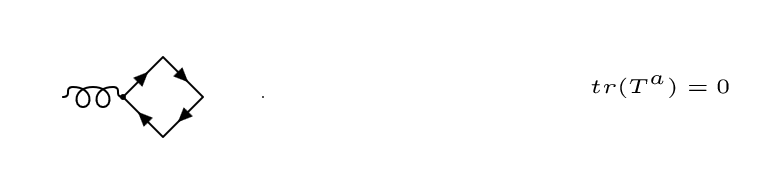
\includegraphics[scale=0.6]{images/Intro/Casimir4.png}
\end{figure}

\item Fierz identity
\end{itemize}
\begin{equation}
\displaystyle\sum\limits_{a} {T_{ij}}^a {T_{kl}}^a = \frac{1}{2}(\delta_{il}\delta_{kj}-\frac{1}{N}\delta_{ij}\delta_{kl})
\label{Fierz}
\end{equation}
With this identity is clarified the difference between QED and QCD. The charge transfer in QED takes place along the Fermion line because photons cannot transport charges. On the other hand, the gluons transfer color charges. 
\begin{figure}[h!]
\centering
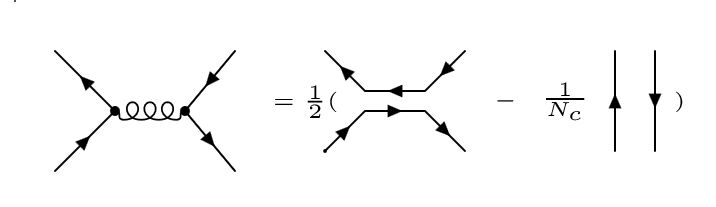
\includegraphics[scale=0.6]{images/Intro/Fritz.png}
\end{figure}
 

Other useful relation for the calculation of casimir operators in SU(N):
\begin{equation}
tr(T^a T^b)= {T_{ij}}^a {T_{ji}}^b = T_F \delta^{ab}
\end{equation}
\begin{equation}
\displaystyle\sum\limits_{a} (T^a T^a) = C_F \delta^{ij}
\end{equation}
\begin{equation}
f^{acd} f^{bcd} = C_A \delta^{ab}
\end{equation}
With $  T_F = \frac{1}{2} $ , $ C_A = N $ and $ C_F = \frac{N^2 -1}{2N} $



\newpage